\documentclass[10pt, a4paper,spanish]{article}
\usepackage[utf8]{inputenc}

\usepackage{lipsum} % Package to generate dummy text throughout this template
\usepackage{varwidth}
\usepackage{hyperref}
\usepackage{graphicx}

\usepackage[T1]{fontenc} % Use 8-bit encoding that has 256 glyphs
\usepackage{microtype} % Slightly tweak font spacing for aesthetics

\usepackage[hmarginratio=1:1,top=32mm,columnsep=20pt]{geometry} % Document margins
\usepackage[hang, small,labelfont=bf,up,textfont=it,up]{caption} % Custom captions under/above floats in tables or figures
\usepackage{booktabs} % Horizontal rules in tables
\usepackage{float} % Required for tables and figures in the multi-column environment - they need to be placed in specific locations with the [H] (e.g. \begin{table}[H])
\usepackage{hyperref} % For hyperlinks in the PDF

\usepackage{lettrine} % The lettrine is the first enlarged letter at the beginning of the text
\usepackage{paralist} % Used for the compactitem environment which makes bullet points with less space between them

\usepackage{abstract} % Allows abstract customization
\renewcommand{\abstractnamefont}{\normalfont\bfseries} % Set the "Abstract" text to bold
\renewcommand{\abstracttextfont}{\normalfont\small\itshape} % Set the abstract itself to small italic text

\usepackage{titlesec} % Allows customization of titles
\renewcommand\thesection{\Roman{section}} % Roman numerals for the sections
\renewcommand\thesubsection{\Roman{subsection}} % Roman numerals for subsections
\titleformat{\section}[block]{\large\scshape\centering}{\thesection.}{1em}{} % Change the look of the section titles
\titleformat{\subsection}[block]{\large}{\thesubsection.}{1em}{} % Change the look of the section titles

\usepackage{fancyhdr} % Headers and footers
\pagestyle{fancy} % All pages have headers and footers
\fancyhead{} % Blank out the default header
\fancyfoot{} % Blank out the default footer
\fancyhead[C]{ Marzo 2016 $\bullet$ Propuesta de Grupo} % Custom header text
\fancyfoot[RO,LE]{\thepage} % Custom footer text

%----------------------------------------------------------------------------------------
%	TITLE SECTION
%----------------------------------------------------------------------------------------

\title{\vspace{-15mm}\fontsize{24pt}{10pt}\selectfont\textbf{Propuesta de Grupo}} % Article title

\author{
\large
\textsc{Alberto Amigo Alonso\textsubscript{25\%}}\\[2mm] % Your name
\textsc{Sergio Delgado Álvarez\textsubscript{25\%}}\\[2mm] % Your name
\textsc{Sergio García Prado\textsubscript{25\%}}\\[2mm] % Your name
\textsc{Oscar Fernández Angulo\textsubscript{25\%}}\\[2mm] % Your name
\normalsize Universidad de Valladolid \\ % Your institution
\vspace{-5mm}
}
\date{}

%----------------------------------------------------------------------------------------

\begin{document}

	\maketitle % Insert title

	\thispagestyle{fancy} % All pages have headers and footers

%----------------------------------------------------------------------------------------
%	ABSTRACT
%----------------------------------------------------------------------------------------

	\begin{abstract}
		\noindent Servicio web destinado a permitir a remitentes y destinatarios ofertar envíos para que los transportistas sean capaces de encontrarlos permitiendo a todos los usuarios monitorizarlos.
	\end{abstract}

%----------------------------------------------------------------------------------------
%	TEXT
%----------------------------------------------------------------------------------------

		\section{Descripción del Problema}

			\paragraph{}
			El transporte es una actividad del sector terciario, entendida como el desplazamiento de objetos o personas de un lugar (punto de origen) a otro (punto de destino) en un vehículo (medio o sistema de transporte) que utiliza una determinada infraestructura (red de transporte). Esta ha sido una de las actividades terciarias que mayor expansión ha experimentado a lo largo de los últimos dos siglos, debido a la industrialización; al aumento del comercio y de los desplazamientos humanos tanto a escala nacional como internacional; y los avances técnicos que se han producido y que han repercutido en una mayor rapidez, capacidad, seguridad y menor coste de los transportes. \cite{wikipedia_transporte}

			\paragraph{}
			Nosotros nos centraremos en el transporte de mercancías para la realización de esta propuesta. En este sector existen tres roles bien diferenciados: el \textbf{remitente}, el \textbf{transportista} y el \textbf{destinatario}. El modelo de negocio actual se basa en empresas intermediarias denominadas \textit{agencias de transporte} cuya labor es poner en contacto remitentes con transportistas que lleven la mercancía hasta su destino.

			\paragraph{}
			Dependiendo de la manera en que se contrate el transporte existen dos formas de pago: por parte del remitente, del destinatario. Actualmente el método más utilizado es el de pago por parte del destinatario pero existen casos especiales en los que no es así. También existen dos métodos de calcular el precio del transporte: aplicando una tarifa fija (lo cual muchas veces infla los costes de manera innecesaria) o por contra, teniendo en cuenta la distancia recorrida desde el origen hasta el destino. Uno de los problemas actuales es el de calcular penalizaciones y recompensas por el tiempo de transporte así como el periodo de tiempo que transcurre durante la carga y descarga de la mercancía.

			\paragraph{}
			La solución que se propone es la creación de un servicio encargado de conectar a transportistas con remitentes y destinatarios de manera eficiente y automática tratando de minimizar los costes entre intermediarios, dando lugar a un mayor beneficio para el transportista y un menor coste para el cliente. En la siguiente sección se describirá más detalladamente tanto las acciones como la descripción de cada uno de los usuarios objetivo.

			\paragraph{}
			Dado que el sistema tratará de llegar al mayor número de personas posibles trataremos de hacer que la interfaz de usuario sea lo más simple posible.
			Se pretende que los usuarios comprendan cómo utilizar el sistema sin importar su edad ni conocimientos informáticos ya que los sectores a los que va destinado el sistema son muy heterogéneos. Por tanto será un punto muy importante tratar de mostrar el mayor número información posible sin sacrificar la facilidad de uso.

			\paragraph{}
			El servicio seguirá una idea similar a la de Uber \copyright\  con el transporte de pasajeros pero aplicado al campo de las mercancías (siempre siguiendo la vigente normativa). Ya existen algunas start-ups que pretenden hacerse un hueco en este nicho de mercado entre las que destacan Convoy \copyright\ y Trucker Path \copyright\ las cuales se basan en una aplicación para sistemas móviles. \cite{expansion_uber_transporte}

			\paragraph{}
			Los usuarios del sistema podran realizar las siguientes acciones:

			\begin{itemize}

				\item Los usuarios se registran en el sistema diferenciando su rol (cliente o transportista)

				\item Los clientes pueden crear envíos en el sistema para que los transportistas les oferten un precio por llevarlo a cabo.

				\item Los clientes seleccionarán al transportista que deseen de entre los que hayan pujado por la oferta de envío.

				\item Una vez confirmado el envío los clientes pueden monitorizar el envío

				\item Los transportistas pueden buscar envíos aplicando los filtros que crean convenientes (localizacion, fecha, etc).

				\item Todos los usuarios del sistema pueden notificar sobre hitos sucedidos en los envíos así como introducir comentarios, lo que fomenta la retroalimentación entre los involucrados.

				\item Los clientes y transportistas tendrán acceso a estadísticas sobre envíos anteriores.


			\end{itemize}



		\section{Usuarios Objetivo}

			\paragraph{}
			Los usuarios objetivo del sistema se dividen en dos grupos bien diferenciados:

			\begin{itemize}


				\item{\textbf{Transportista}}

				\paragraph{}
				El transportista es la persona encargada de llevar el envío desde el lugar de origen hasta el de destino.

				\paragraph{}
				El sistema, por tanto, tendrá la labor de permitirle encontrar envíos que se ajusten a las requisitos que el transportista requiera como localización del punto de partida, del de llegada, fecha, tipo de transporte, etc. Una vez que el transportista encuentre un envío que pretenda realizar deberá fijar un precio por el cual estaría dispuesto a llevarlo a cabo. A partir de este punto deberá esperar la confirmación del cliente para dirigirse al punto de partida.

				\paragraph{}
				Además de esto, el sistema también ofrecerá al transportista la posibilidad de notificar hitos al cliente tales como que su envío a sufrido algún contratiempo o que se ha completado cierta distancia.

				\paragraph{}
				El transportista también tendrá la posibilidad de acceder a información de anteriores envíos así como estadísticas sobre los destinos y orígenes, zonas donde se le han aceptado pujas más altas, etc.


				\item{\textbf{Cliente}}
				\paragraph{}
				El rol de cliente es el cliente. Este será quien oferte envíos a realizar en el sistema. Dentro de este se agrupan los dos clientes implicados en ello, es decir, el remitente y el destinatario. Estos roles no son fijos sino que se fijarán en cada envío según sea pertinente.

				\paragraph{}
				No existe restricción acerca de quién de los dos es el encargado de crear el envío, sino que habrá casos en los cuales serán los remitentes los que deseen enviar algo. También habrá casos en los cuales el destinatario es quien solicitará que se vaya a recoger mercancia a un lugar concreto.

				\paragraph{}
				El cliente que introduzca el envío en el sistema será también el encargado tanto de realizar el pago como de seleccionar el transportista que más desee de entre los que hayan pujado.

				\paragraph{}
				Ahora describiremos más detalladamente cada uno de los subroles:

				\begin{itemize}

					\item{\textbf{Remitente}}
					\paragraph{}
					El remitente será la persona encargada de suministrar la mercancia al transportista para que la lleve hasta el destinatario. El remitente podrá fijar una hora preferida de recogida dado que podría no estar disponible cuando el transportista llegue a recogerlo.

					\item{\textbf{Destinatario}}
					\paragraph{}
					El destinatario será la persona encargada de recoger el envío en el lugar de destino al cual llegará el transportista. El destinatarío podrá fijar una hora preferida de entrega dado que podría no estar disponible cuando el transportista llegue a entregarlo.

				\end{itemize}





			\end{itemize}
		\section{Borrador de la Solución}

			\paragraph{}
			La estructura de navegación por la página web será de scroll infinito siguiendo la idea que actualmente están llevando a cabo las principales redes sociales como Facebook \copyright y  Twitter \copyright. Hemos escogido esta idea en vez de la navegación por pestañas de la propuesta individual porque creemos que será más sencillo de utilizar para la mayoría de los usuarios.

			\paragraph{}
			A continuación procederemos a describir el conjunto de vistas que formarán el servicio web. Dado que existen dos roles bien diferenciados (cliente y transportista) las vistas que sean comunes a los dos pero tengan pequeñas diferencias se describirán juntas explicando dichas variaciones.

			\begin{figure}[H]
				\centering
				\begin{minipage}[b]{0.8\textwidth}
					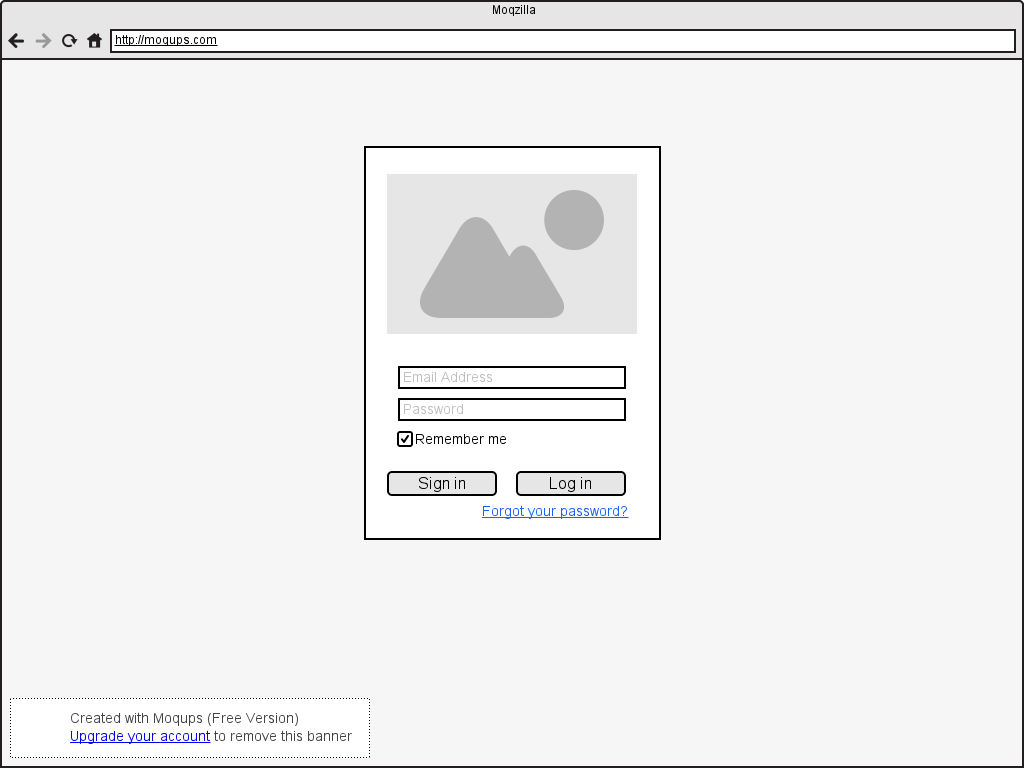
\includegraphics[width=\textwidth]{res/Login.png}
				\end{minipage}
			\end{figure}

			\paragraph{}
			La vista de \textbf{login} será lo primero que el usuario visualizará al acceder al sitio web, en esta parte se identificará o creará una cuenta en el caso de que no la tuviera todavía.


			\begin{figure}[H]
				\centering
				\begin{minipage}[b]{0.49\textwidth}
					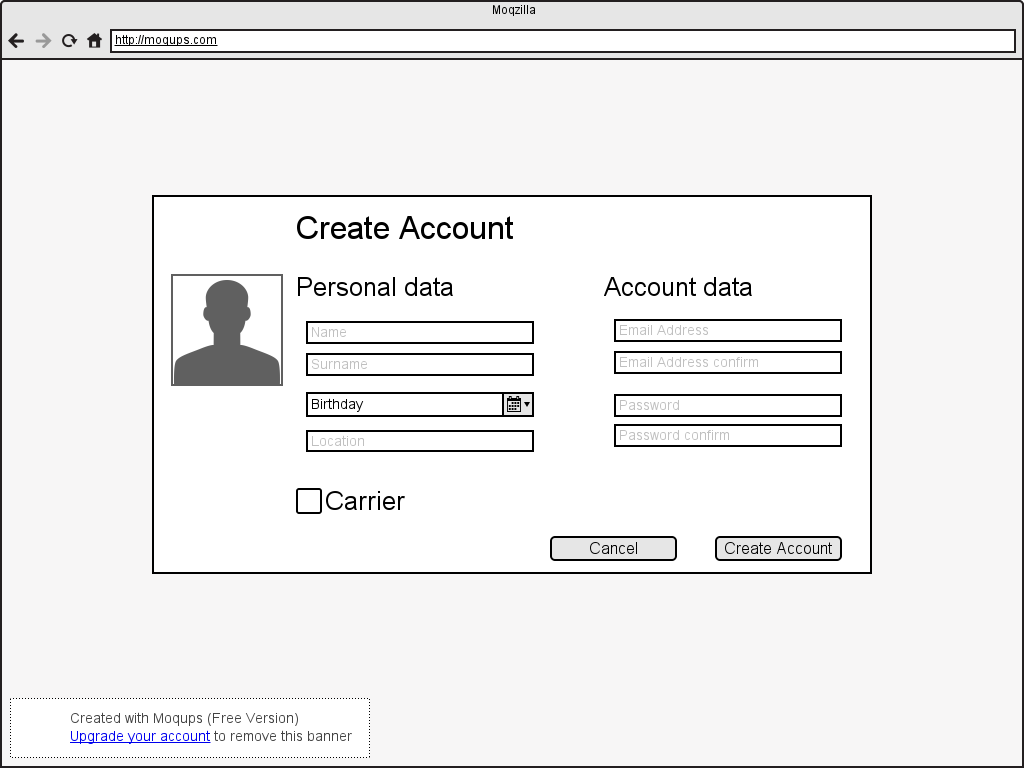
\includegraphics[width=\textwidth]{res/CrearCuenta.png}
				\end{minipage}
				\begin{minipage}[b]{0.49\textwidth}
					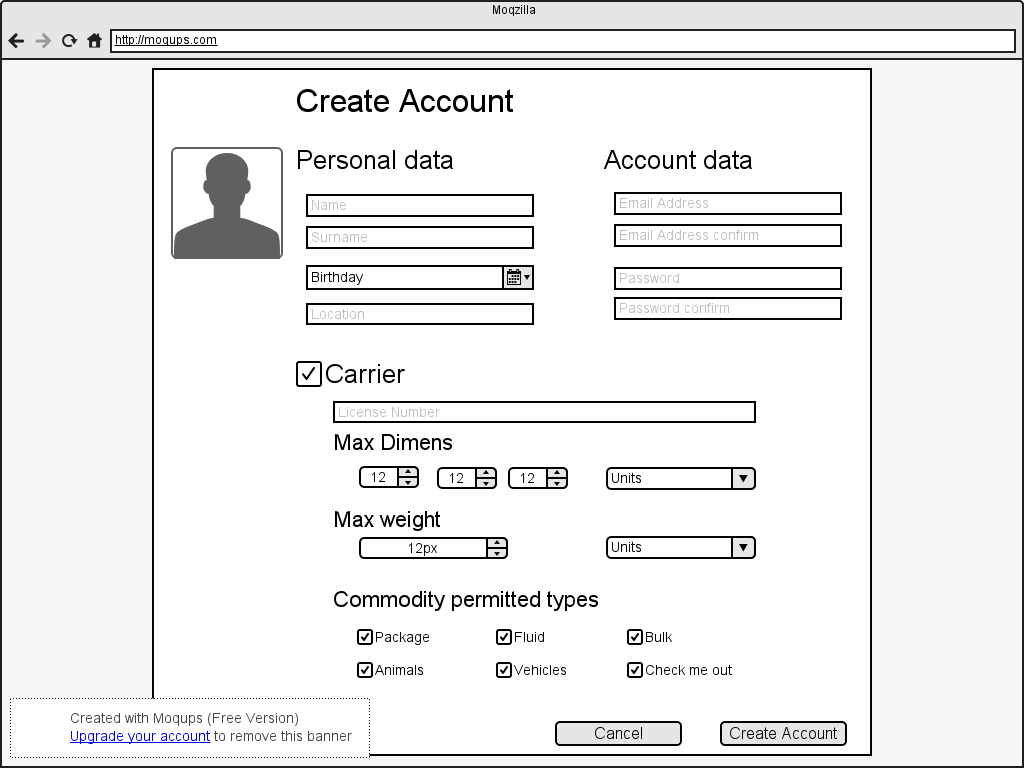
\includegraphics[width=\textwidth]{res/CrearCuentaTransportista.png}
				\end{minipage}
			\end{figure}

			\paragraph{}
			En la vista de \textbf{crear cuenta} es donde el usuario introducirá sus datos personales. Esta parte será común para los dos roles. Además habrá un checkbutton que el usuario deberá marcar en el caso de que sea transportista. Entonces en la vista aparecerán nuevos campos donde este deberá introducir las caracteristicas de su método de transporte (tamaño, peso máximo, tipo de envíos que puede transportar, etc). En este punto el sistema ya tendrá diferenciados los dos roles.

			\paragraph{}
			Primero describiremos las vistas que el cliente podrá visualizar y luego nos centraremos en las del transportista.

			\begin{figure}[H]
				\centering
				\begin{minipage}[b]{0.8\textwidth}
					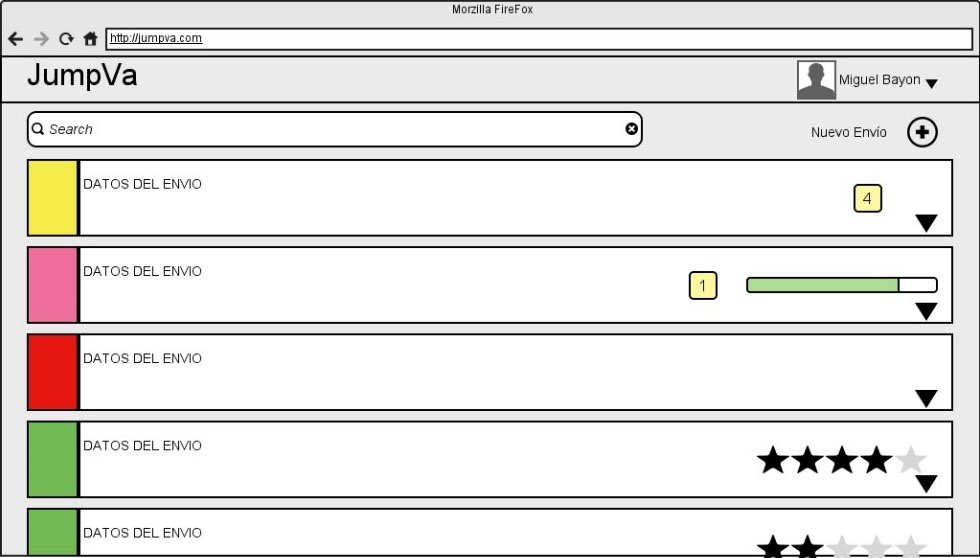
\includegraphics[width=\textwidth]{res/PaginaPrincipal.png}
				\end{minipage}
			\end{figure}

			\paragraph{}
			La vista de \textbf{página principal} del sitio web. Será la que se mostrará al iniciar sesión como remitente en el sitio web. En ella se mostrará al cliente información acerca de los envíos que están en curso, los que están pendientes de confirmación para que los confirme seleccionando el transportista que más desee. También se le mostrarán los envíos ya finalizados para que si lo desea pueda introducir la opinión acerca de anteriores envíos. Esta página tendrá un scroll infinito en el cual se le mostrarán todos los envíos que ha realizado. Además en la parte superior de la página habrá una barra de búsqueda que permitirá filtrar envíos por origenes, destinos, fechas, etc. lo cual permitirá encontrar cualquier envío anterior de manera sencilla. También hay un botón en la parte superior derecha cuya función es la de crear nuevos envíos.


			\begin{figure}[H]
				\centering
				\begin{minipage}[b]{0.49\textwidth}
					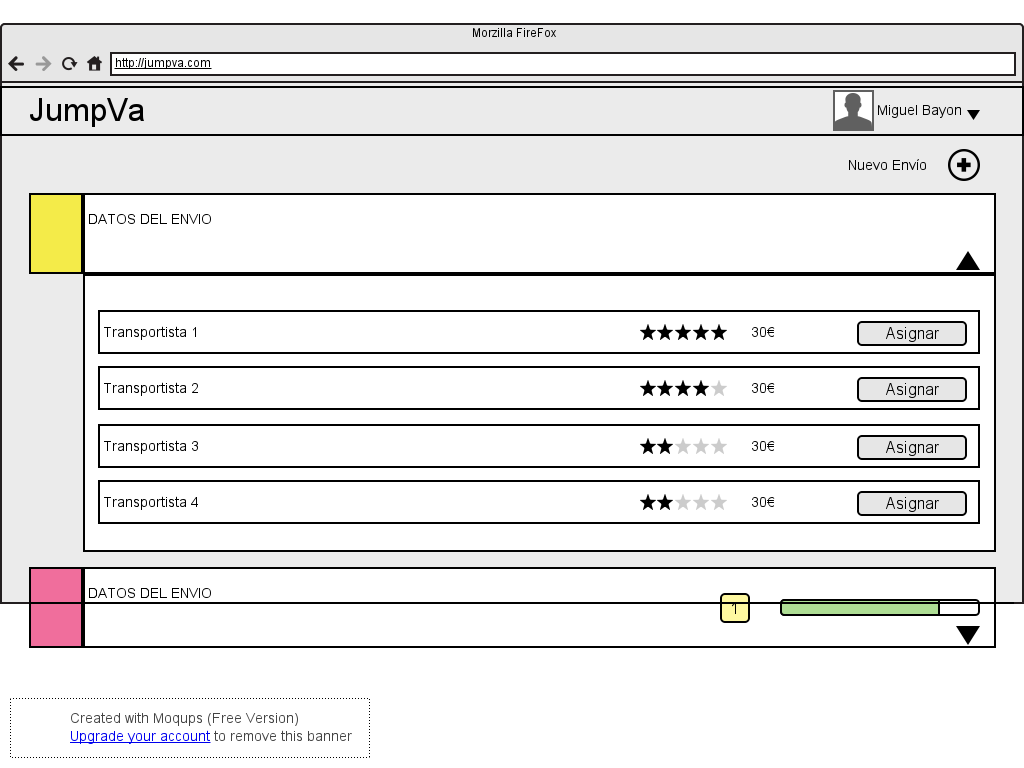
\includegraphics[width=\textwidth]{res/ExpansionEnvioPendienteAsignacion.png}

				\end{minipage}
				\begin{minipage}[b]{0.49\textwidth}
					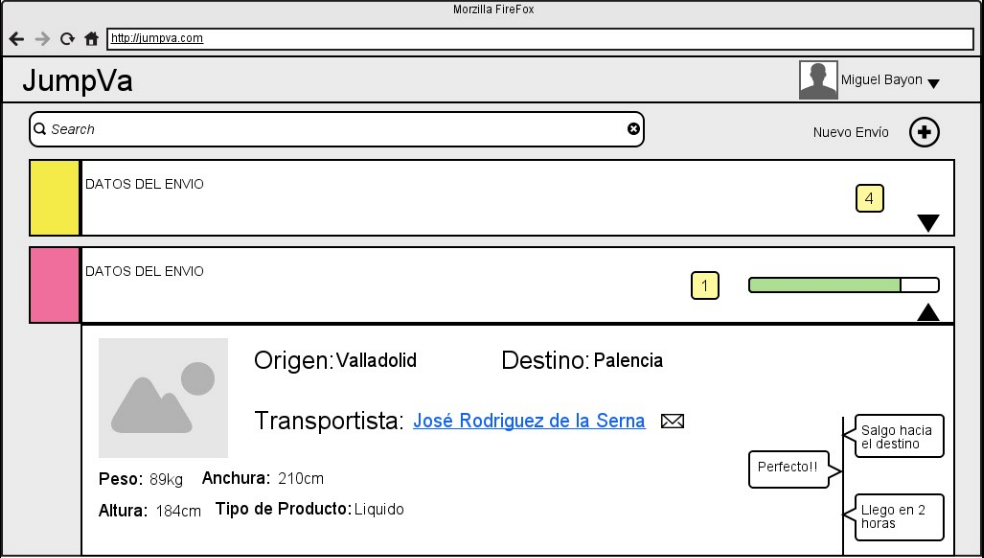
\includegraphics[width=\textwidth]{res/ExpansionEnvioEnProceso.png}
				\end{minipage}
			\end{figure}

			\paragraph{}
			Las dos vistas que se adjuntan en la imagen superior se corresponden con la información que se muestra al clickar (se abre un menu desplegable inferiormente) en los envíos que todavía no están confirmados, y un envío en progreso, este ultimo sera comun para ambos tipos de usuario.


			\begin{figure}[H]
				\centering
				\begin{minipage}[b]{0.49\textwidth}
					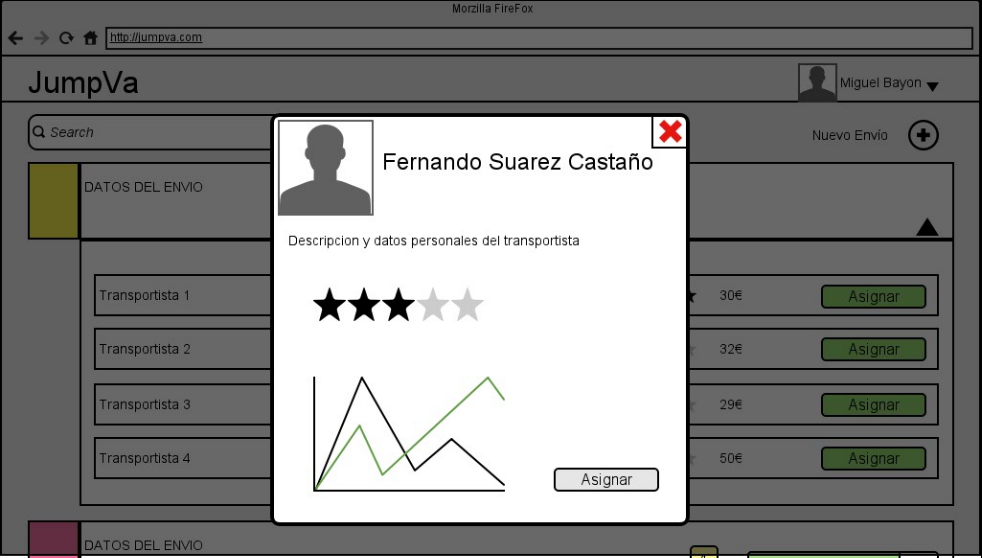
\includegraphics[width=\textwidth]{res/DetallesTransportista.png}

				\end{minipage}
				\begin{minipage}[b]{0.49\textwidth}
					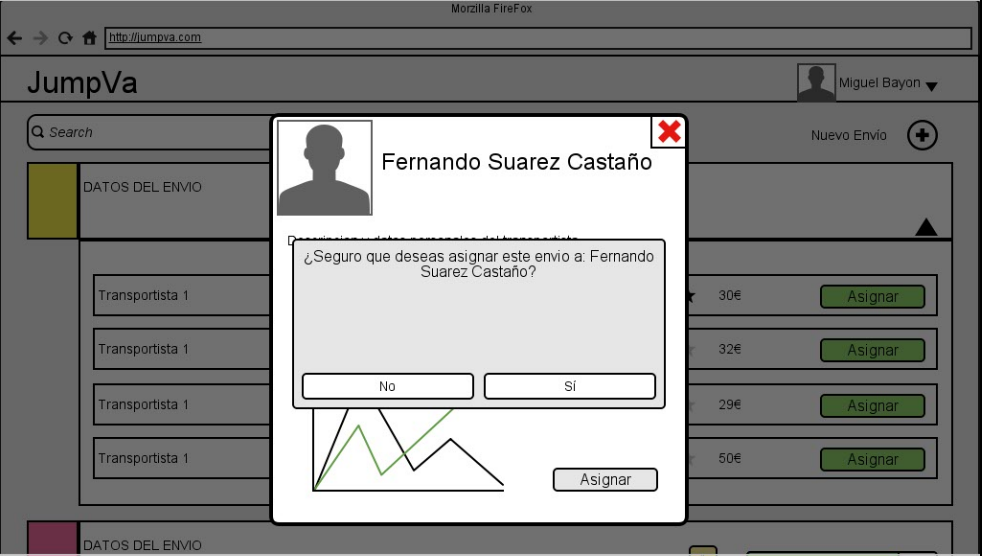
\includegraphics[width=\textwidth]{res/ConfirmacionAsignacion.png}

				\end{minipage}
			\end{figure}

			\paragraph{}
			La imagen superior ilustra el caso de que un cliente consulte el perfil de un transportista y seguidamente quiera confirmar que lo realice ese transportista.

			\begin{figure}[H]
				\centering
				\begin{minipage}[b]{0.49\textwidth}
					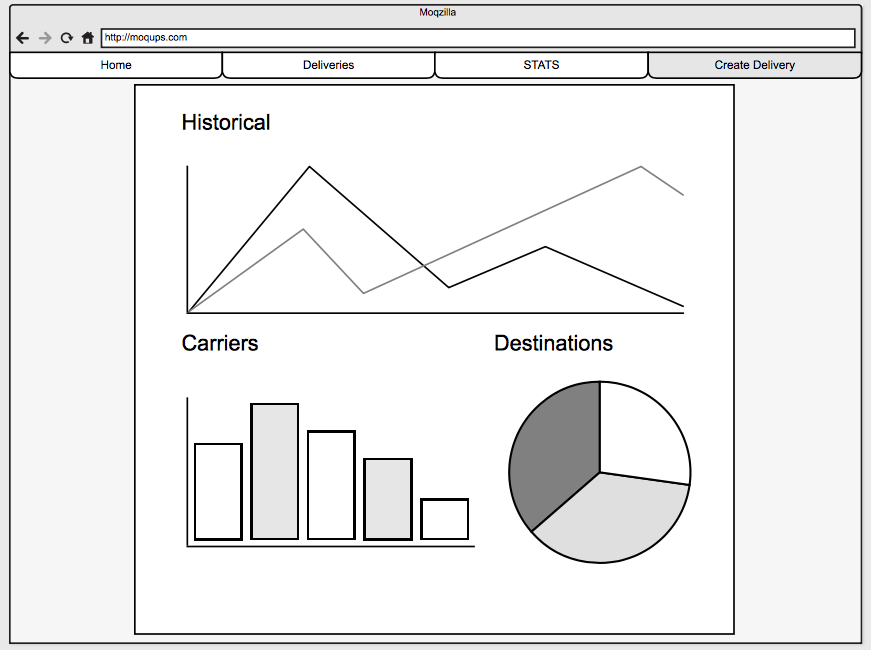
\includegraphics[width=\textwidth]{res/Estadisticas.png}

				\end{minipage}
				\begin{minipage}[b]{0.49\textwidth}
					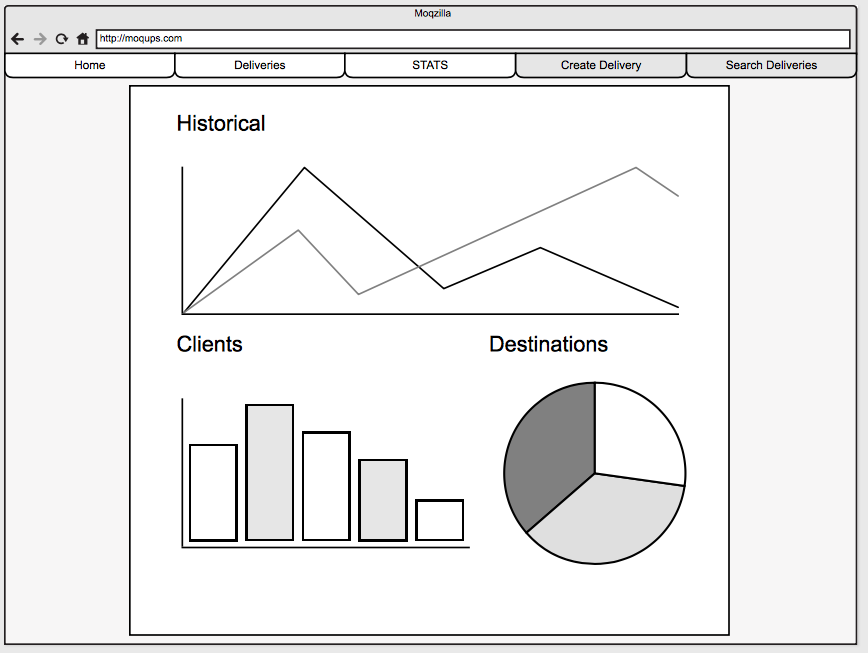
\includegraphics[width=\textwidth]{res/EstadisticasTransportista.png}

				\end{minipage}
			\end{figure}

			\paragraph{}
			La vista de \textbf{estadisticas} servirá para que los usuarios puedan obtener información gráficamente de manera rápida sobre envíos pasados. Tendrán un gráfico de líneas en el cual se mostrará la evolución del número de envíos respecto del tiempo. Además también tendrán otras métricas como el número de veces que han usado el mismo transportista en el caso del cliente y a la inversa en el caso del transportista. También podrán obtener métricas acerca de los orígenes y destinos a los que se han enviado pedidos, etc.

			\paragraph{}
			Las siguientes vistas serán de tipo emergente, es decir, se superpondrán al resto del contenido de la página. Si es posible se intentará hacer sin utilizar ventanas.


			\begin{figure}[H]
				\centering
				\begin{minipage}[b]{0.7\textwidth}
					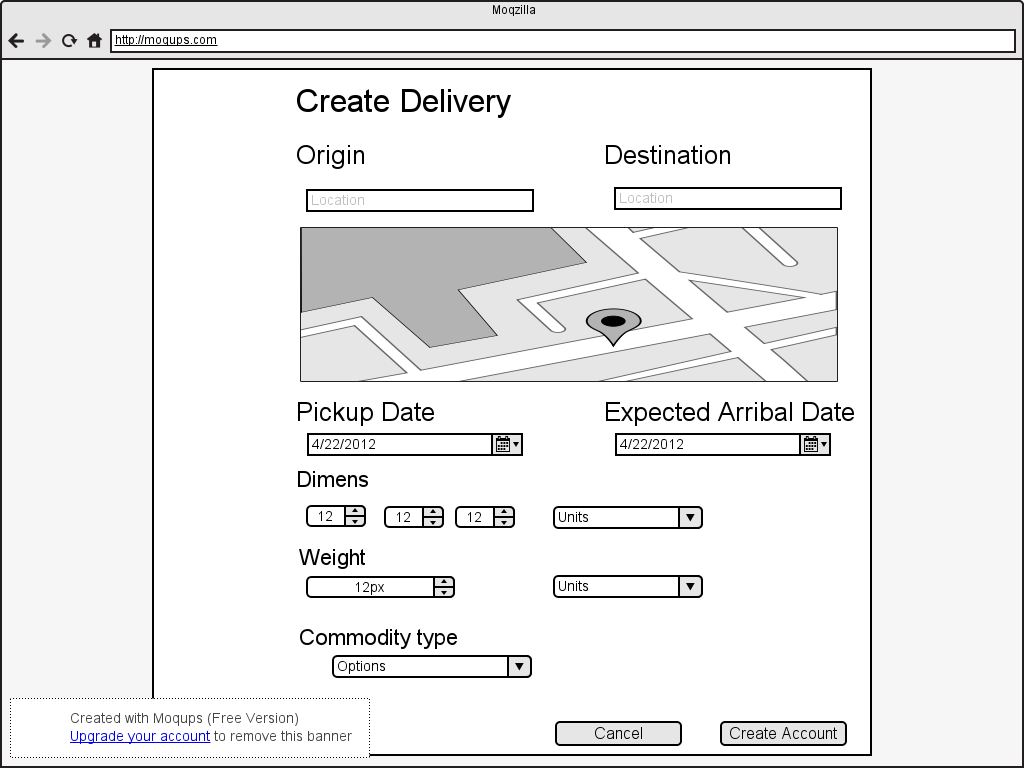
\includegraphics[width=\textwidth]{res/CrearEnvio.png}

				\end{minipage}
			\end{figure}

			\paragraph{}
			La vista de \textbf{crear envío} será única para los clientes. En esta introducirán información acerca de qué quieren enviar, desde dónde hasta dónde, en qué fecha, etc. El cliente además tendrá la posibilidad de introducir imágenes del paquete que después el transportista podrá visualizar antes de solicitar realizar el envío.
			
			\begin{figure}[H]
				\centering
				\begin{minipage}[b]{0.7\textwidth}
					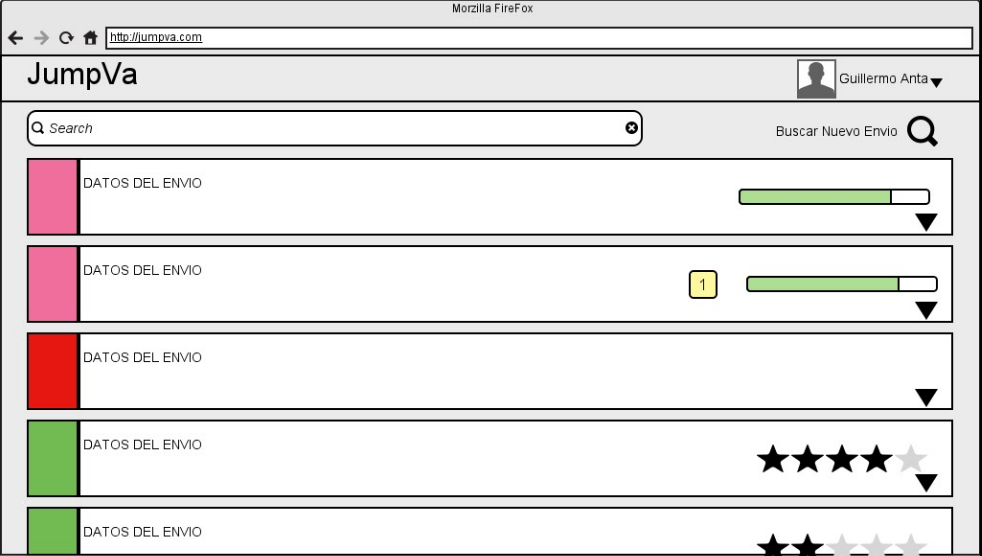
\includegraphics[width=\textwidth]{res/PaginaPrincipalTransportista.png}

				\end{minipage}
			\end{figure}
			
			\paragraph{}
			La vista de \textbf{pagina principal transportista}, sera la pagina principal que se visualizara al iniciar sesion como transportista. Es muy similar a la pagina principal del remitente. En ella el cliente podra consultar todos los envios que esta realizando en este momento, los que ya ha completado... Tambien tendra la posibilidad de buscar un nuevo envio si asi lo desea. Las vistas que se mostraran al hacer click sobre los diferentes envios que aparecen en la pagina principal seran similares a las descritas anteriormente.


			\begin{figure}[H]
				\centering
				\begin{minipage}[b]{0.7\textwidth}
					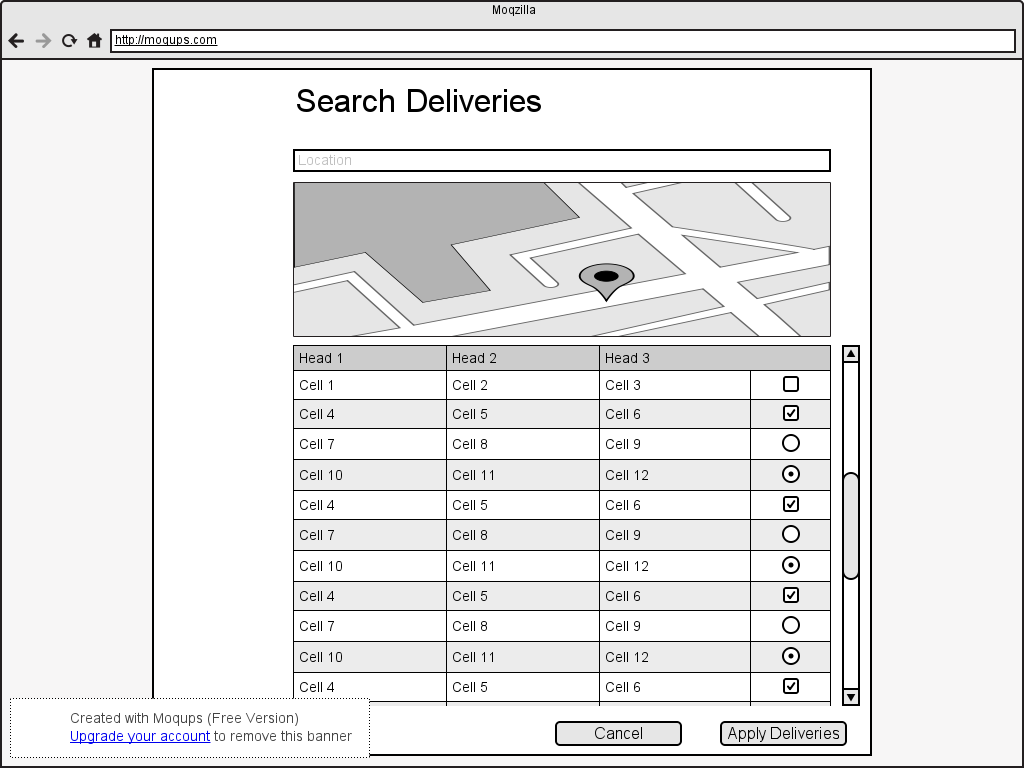
\includegraphics[width=\textwidth]{res/BuscarEnviosTransportista.png}

				\end{minipage}
				\begin{minipage}[b]{0.7\textwidth}
					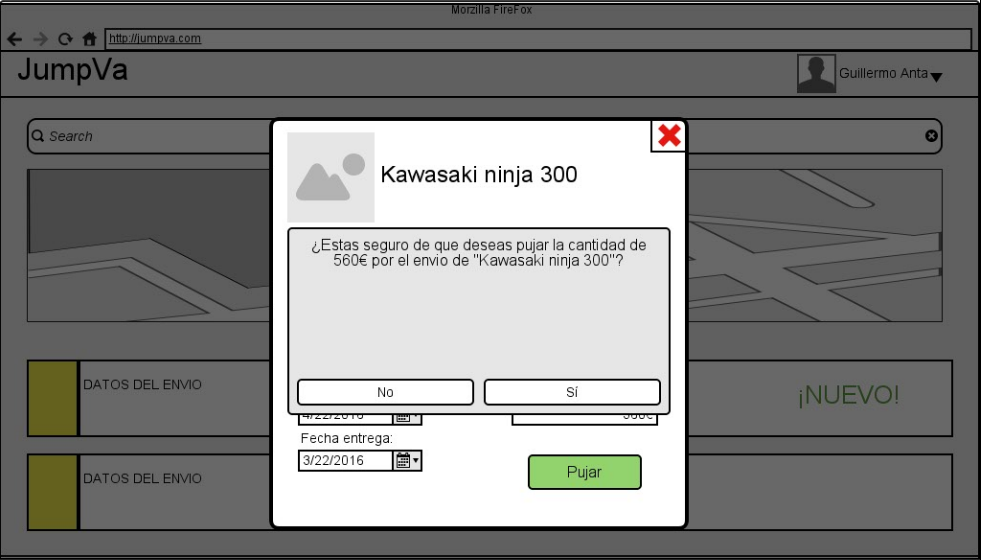
\includegraphics[width=\textwidth]{res/ConfirmacionDePuja.png}

				\end{minipage}
			\end{figure}

			\paragraph{}
			La vista de \textbf{buscar envíos} será única para los transportistas. En esta vista los transportistas introducirán su ubicación actual o utilizaran la barra de busqueda y seguidamente el sistema les devolverá un listado los envíos disponibles más cercanos. Seguidamente el transportista podrá revisar la informacion de los diferentes envios, y si lo desea pujar por aquellos que le interesen.


			\begin{figure}[H]
				\centering
				\begin{minipage}[b]{0.7\textwidth}
					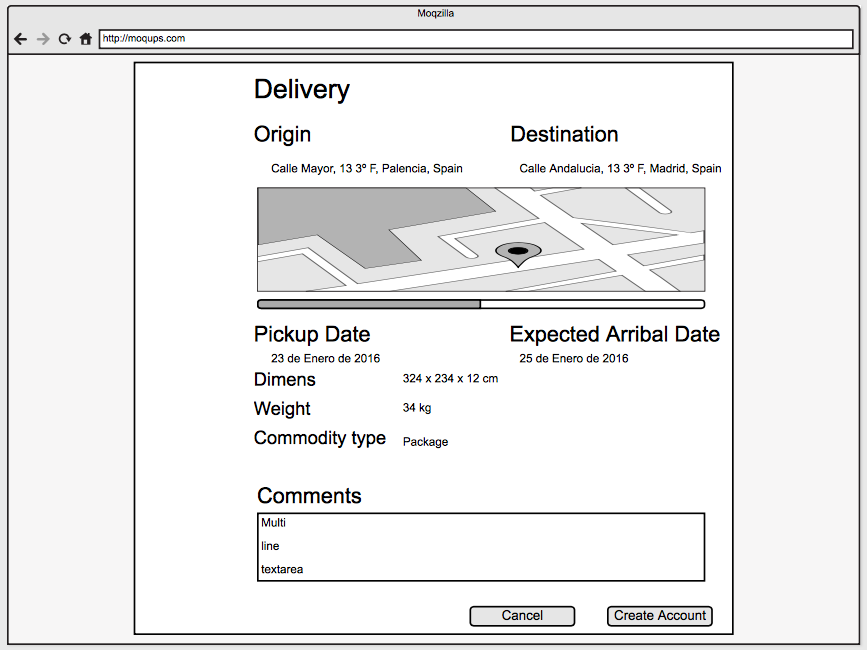
\includegraphics[width=\textwidth]{res/sketch_delivery.png}

				\end{minipage}
			\end{figure}

			\paragraph{}
			La vista de \textbf{envío} se corresponde con la informacion mostrada al hacer click sobre uno de los envios que aparecen listados en la página de busqueda, y en ella el transportista podra realizar una oferta para realizar el envio. La vista de \textbf{confirmar puja} se mostrara para confirmar que la puja introducida por el transportista es la deseada.
			
			\paragraph{}
			Ambas vistas seran de tipo emergente, se superpondran al resto del contenido dejandolo oscurecido en un segundo plano.
%----------------------------------------------------------------------------------------
%	Bibliographic references
%----------------------------------------------------------------------------------------
	\begin{thebibliography}{9}

		\bibitem{wikipedia_transporte}
		Wikipedia. Transporte. \url{https://es.wikipedia.org/wiki/Transporte}

		\bibitem{expansion_uber_transporte}
		Expansión. Se busca el Uber del transporte de mercancías. \url{http://www.expansion.com/economia-digital/2015/10/29/5630ef8e46163f932a8b45d9.html}

	\end{thebibliography}


\end{document}
